\documentclass[scheme = chinese]{ctexart}

% Set page size and margins
% Replace `letterpaper' with`a4paper' for UK/EU standard size
\usepackage[a4paper,top=2cm,bottom=2cm,left=3cm,right=3cm,marginparwidth=1.75cm]{geometry}
% Useful packages
\usepackage{amsmath}
\usepackage{graphicx}
\usepackage[colorlinks=false, allcolors=blue]{hyperref}
\usepackage[final]{pdfpages}
\usepackage{booktabs}
\usepackage{caption}
\usepackage{makecell}
\graphicspath{ {./images/} }
\usepackage{varioref}
\usepackage{float}
\usepackage{listings}
\usepackage{minted}
\usepackage{longtable}
\usepackage{subfiles}
\usepackage[figuresright]{rotating}
\usepackage[graphicx]{realboxes}
\usepackage{adjustbox}
\usepackage{blindtext}


\newcommand*\xor{\oplus}

\begin{document}
\title{VerilogHDL与FPGA完成MIPS微系统开发}
\author{孙天天 19071110}
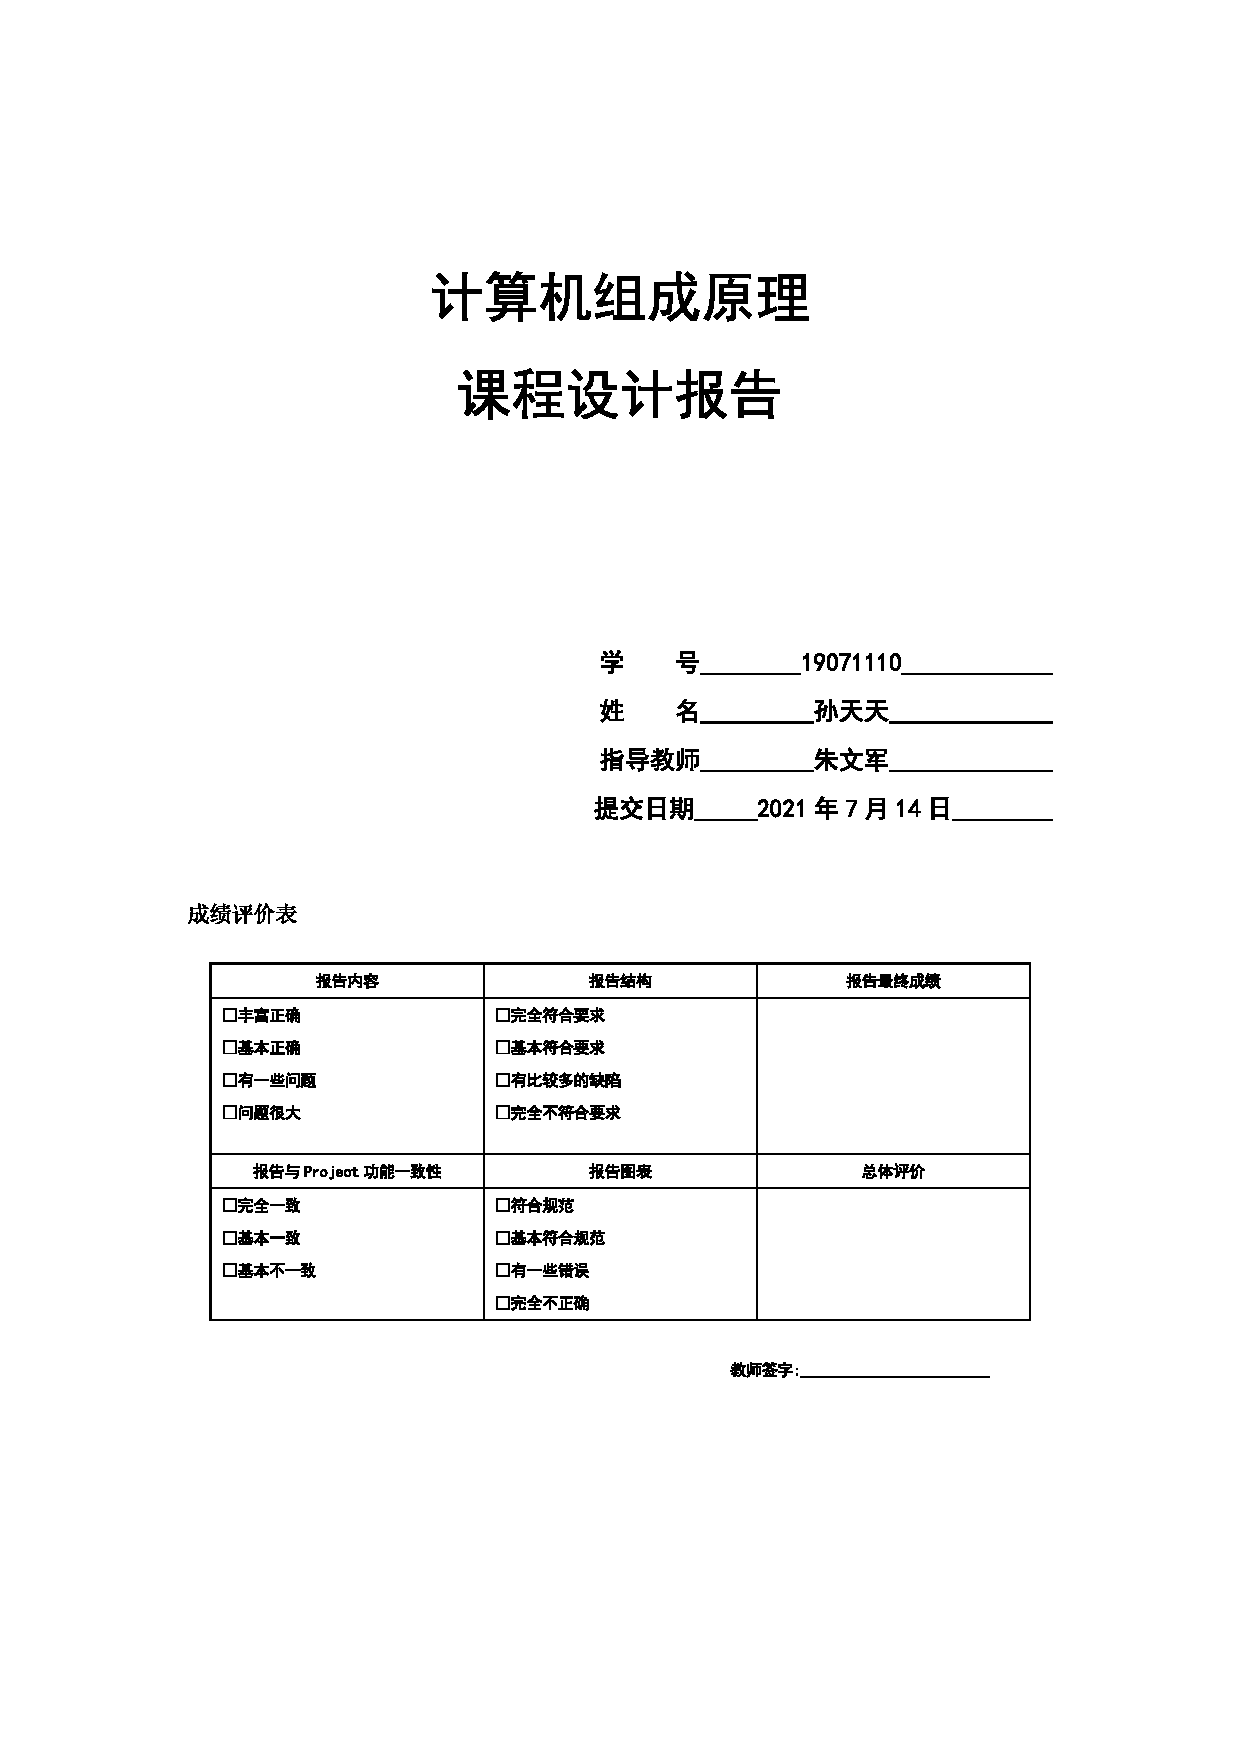
\includepdf[pages=-,pagecommand={},width=\textwidth]{cover.pdf}

\tableofcontents
\clearpage

\maketitle


\part{VerilogHDL完成单周期处理器开发}
\setcounter{section}{0}
\subfile{Project1/section1-overall.tex}
\clearpage
\subfile{Project1/section2-modules.tex}
\clearpage
\subfile{Project1/section3-testing.tex}
\clearpage

\part{VerilogHDL完成多周期处理器开发}
\setcounter{section}{0}
\subfile{Project2/section1-overall.tex}
\clearpage
\subfile{Project2/section2-modules.tex}
\clearpage
\subfile{Project2/section3-testing.tex}
\clearpage

\part{VerilogHDL完成多周期处理器开发(支持设备与中断)}
\setcounter{section}{0}
\subfile{Project3/section1-overall.tex}
\clearpage
\subfile{Project3/section2-modules.tex}
\clearpage
\subfile{Project3/section3-testing.tex}
\clearpage

\part{FPGA完成多周期处理器开发(支持设备与中断)}
\setcounter{section}{0}
\subfile{Project4/section1-overall.tex}
\clearpage
\subfile{Project4/section3-testing.tex}
\clearpage

\part{机器指令描述}
助记码、操作码、功能
\begin{center}
    \captionof{table}{各指令的状态循环节}
    \begin{tabular}{cccccccc}
        \toprule
        助记码 & opcode & funct & CP0Funct & 功能 \\
        \midrule
        addu & 0b000000 & 0b100001 & - & 无符号加法 \\
        subu & 0b000000 & 0b100011 & - & 无符号减法 \\
        ori & 0b001101 & - & - & 立即数按位或 \\
        lw & 0b100011 & - & - & 从内存读取字 \\
        sw & 0b101011 & - & - & 向内存写入字 \\
        beq & 0b000100 & - & - & 分支判断是否相等 \\
        j & 0b000010 & - & - & 跳转 \\
        lui & 0b001111 & - & - & 高位载入 \\
        addi & 0b001000 & - & - & 立即数加法 \\
        addiu & 0b001001 & - & - & 无符号立即数加法 \\
        slt & 0b000000 & 0b101010 & - & 有符号比较 \\
        nop & 0b000000 & 0b000000 & - & 无操作 \\
        lb & 0b100000 & - & - & 从内存读取字节 \\
        sb & 0b101000 & - & - & 向内存写入字节 \\
        jal & 0b000011 & - & - & 跳转并连接 \\
        jr & 0b000000 & 0b001000 & - & 返回 \\
        eret & 0b010000 & - & 0b011000 & 中断返回 \\
        mfc0 & 0b010000 & - & 0b00000 & 从CP0读取 \\
        mtc0 & 0b010000 & - & 0b00100 & 向CP0写入 \\
        \bottomrule
    \end{tabular}
\end{center}
\clearpage

\part{总结与收获}
\setcounter{section}{0}
\subfile{section4-summary.tex}
\clearpage

\end{document}